\usetikzlibrary{calc}

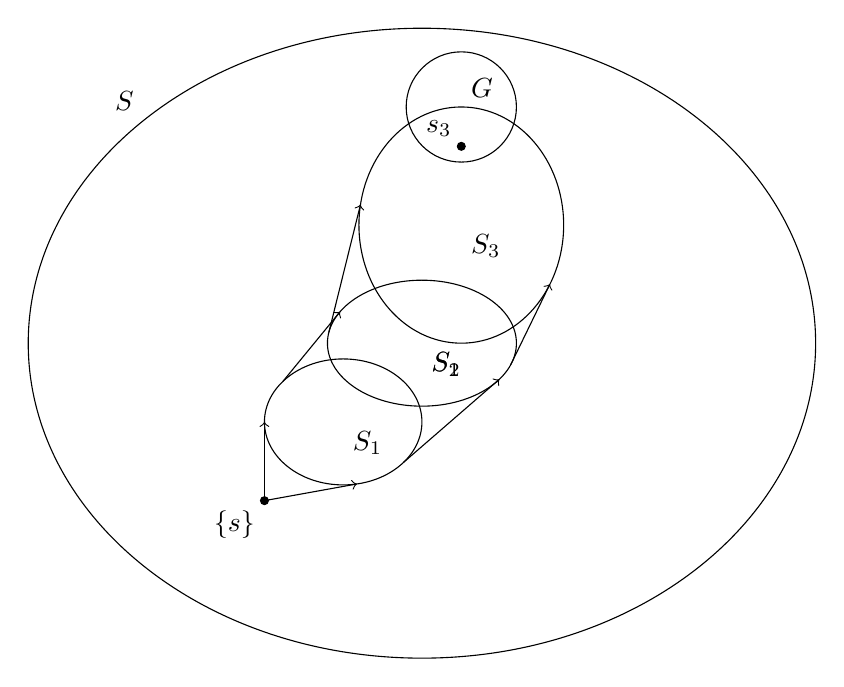
\begin{tikzpicture}

\draw (2,2) node[below right]  {$S_1$} ellipse (5 and 4);
\node[above left] (S) at ($(2,2) + (135:5 and 4)$) {$S$};

\draw[fill] (0,0) node[below left] (S) {$\{s\}$} circle (.05); 

\draw (1,1) node[below right]  {$S_1$} ellipse (1 and .8); 
\draw[->] (0,0) -- ($(1,1) + (180:1 and .8)$);
\draw[->] (0,0) -- ($(1,1) + (-80:1 and .8)$);

\draw (2,2) node[below right]  {$S_2$} ellipse (1.2 and .8); 
\draw[->] ($(1,1) + (140:1 and .8)$) -- ($(2,2) + (150:1.2 and .8)$);
\draw[->] ($(1,1) + (-40:1 and .8)$) -- ($(2,2) + (-35:1.2 and .8)$);

\draw (2.5,3.5) node[below right]  {$S_3$} ellipse (1.3 and 1.5); 
\draw[->] ($(2,2) + (170:1.2 and .8)$) -- ($(2.5,3.5) + (170:1.3 and 1.5)$);
\draw[->] ($(2,2) + (-20:1.2 and .8)$) -- ($(2.5,3.5) + (-30:1.3 and 1.5)$);

\draw (2.5,5) node[above right]  {$G$} circle (.7);

\draw[fill] (2.5,4.5) node[above left] {$s_3$} circle (.05); 
\end{tikzpicture}